
\section{Diagramy. Ruchy Reidemeistera}

Chociaż w~świetle definicji \ref{def:knot} węzły są pewnymi regularnymi podzbiorami przestrzeni $\R^3$, z~kombinatorycznego punktu widzenia wygodniej jest rysować je na płaszczyźnie.

% DICTIONARY;shadow;cień;-
\begin{definition}
\index{cień}%
    Rzut węzła $K \subseteq \R^3$ na płaszczyznę nazywamy cieniem.
\end{definition}

% DICTIONARY;crossing;skrzyżowanie;-
\begin{definition}[skrzyżowanie]
\label{def:crossing}%
\index{skrzyżowanie}%
    Podwójny punkt w cieniu nazywamy skrzyżowaniem.
\end{definition}

% DICTIONARY;diagram;diagram;-
\begin{definition}[diagram]
\index{diagram}%
    Cień razem z~informacją o~tym, jak przebiegają skrzyżowania i pozbawiony katastrof: potrójnych przecięć, stycznych czy dziobów nazywamy diagramem.
    % TODO: Narysować katastrofy
\end{definition}

Dla każdego ustalonego $n \ge 2$ i każdego węzła $K$ istnieje cień $D$, na którym wszystkie wielokrotne punkty są $n$-krotne (wiemy to od Hostego, College'a \cite[s. 11]{adams2021}, którzy nie napisali, skąd to wiedzą);
\index[persons]{Hoste, Jim}%
\index[persons]{College, Pitzer}%
dla co najmniej jednej wartości $n$ można dodatkowo wymagać, by diagram zawierał dokładnie jedno skrzyżowanie (Adams, Crawford, DeMeo, Landry, Lin, Montee, Park, Venkatesh, Yhee \cite{venkatesh2015} albo Brunn\footnote{Karl Hermann Brunn opisał w 1892 roku sploty Brunna, a więc zanim jeszcze teoria węzłów przyszła na świat.} ponad sto lat temu \cite[s. 28]{adams2021}!).
\index[persons]{Adams, Colin}%
\index[persons]{Crawford, Thomas}%
\index[persons]{DeMeo, Benjamin}%
\index[persons]{Landry, Michael}%
\index[persons]{Lin, Alex}%
\index[persons]{Montee, Murphy}%
\index[persons]{Park, Seojung}
\index[persons]{Venkatesh, Saraswathi}%
\index[persons]{Yhee, Farrah}%

\begin{definition}[włókno]
\index{włókno}%
    Fragment diagramu, który biegnie między dwoma kolejnymi tunelami, czyli podskrzyżowaniami, nazywamy włóknem.
\end{definition}

\begin{definition}[nić]
\index{nić}%
    Fragment diagramu, który biegnie między dwoma kolejnymi skrzyżowaniami, nazywamy nicią.
\end{definition}

Nici powstają z włókien przez rozcięcie ich przy każdym nadskrzyżowaniu.

\begin{proposition}
\label{prp:links_have_diagrams}%
    Niech $L$ będzie splotem.
    Jego diagramy tworzą otwarty i~gęsty podzbiór wszystkich rzutów.
\end{proposition}

Kawauchi \cite[s. 7]{kawauchi1996} wspomina w tym miejscu podręcznik Crowella, Foxa \cite[s. 7]{crowell1963}.
To samo jest na przykład u Burdego, Zieschanga, Heusenera \cite[s. 10]{burde2014}, ale oni odsyłają jeszcze do Reidemeistera \cite{reidemeister1927} i samego Burdego \cite{burde1978}.

\begin{proof}[Niedowód]
    Rzut splotu na równoległe płaszczyzny jest taki sam, a te można sparametryzować prostymi przechodzącymi przez początek układu współrzędnych, które tworzą przestrzeń rzutową $\R \mathbb P^2$.
    Niech $S$ będzie zbiorem prostych, które dają złe rzuty.
    Wystarczy pokazać jego nigdziegęstość.
    Okazuje się, że $S$ jest też jednowymiarowy.
\end{proof}

\begin{corollary}
    Każdy splot posiada diagram.
\end{corollary}

% DICTIONARY;oriented;zorientowany;węzeł
\begin{definition}[orientacja]
\index{węzeł!zorientowany}%
\index{orientacja|see {węzeł zorientowany}}%
    Węzeł, w~którym wybrano kierunek, w~którym należy się po nim poruszać, nazywamy zorientowanym.
    Splot nazywamy zorientowanym, jeśli wszystkie jego ogniwa traktowane jako węzły są zorientowane.
\end{definition}

Orientację na diagramie zaznaczamy małą strzałką wskazującą kierunek poruszania się.


\subsection{Ruchy Reidemeistera}

Wiemy już, że węzły mają wiele diagramów.
Mając dane dwa różne diagramy chcielibyśmy wiedzieć, czy przedstawiają ten sam węzeł.
Stosowne narzędzie dostarczył Kurt Reidemeister w~latach dwudziestych ubiegłego wieku.
\index[persons]{Reidemeister, Kurt}%
Zdefiniujmy trzy lokalne operacje na diagramach, a~potem wysłowimy kryterium  Reidemeistera rozstrzygające problem równości węzłów.

% DICTIONARY;Reidemeister/Turaev/... move;ruch Reidemeistera/Turajewa/...;-
\begin{definition}[ruchy Reidemeistera]
\index{ruch!Reidemeistera}%
    Trzy gatunki lokalnych deformacji diagramu splotu:
    \begin{figure}[H]
    \centering
    \begin{minipage}[b]{.22\linewidth}%
        \centering%
        \MedLarReidemeisterOneLeft $\stackrel{R_1}{\cong}$ \MedLarReidemeisterOneStraight%
        \subcaption{ruch $R_1$}%
    \end{minipage}
    \quad\quad\quad
    \begin{minipage}[b]{.2\linewidth}
        \centering
        \MedLarReidemeisterTwoA $\stackrel{R_2}{\cong}$ \MedLarReidemeisterTwoB
        \subcaption{ruch $R_2$}
    \end{minipage}
    \quad\quad\quad
    \begin{minipage}[b]{.32\linewidth}
        \centering
        \MedLarReidemeisterThreeA $\stackrel{R_3}{\cong}$ \MedLarReidemeisterThreeB
        \subcaption{ruch $R_3$}
    \end{minipage}
    \caption[reidemeister-moves]{Trzy ruchy Reidemeistera}
    \end{figure}
    nazywamy ruchami Reidemeistera.
    Czasami używa się konkretnych nazw:
    \begin{itemize}
        \item skręcenie/rozkręcenie (dla $R_1$),
        \item wsunięcie/rozsunięcie (dla $R_2$) oraz
        \item przesunięcie łuku przez skrzyżowanie (dla $R_3$).
    \end{itemize}
\end{definition}

Reidemeister w~swojej pierwszej pracy przyjął inną kolejność, jego drugi ruch jest naszym pierwszym.
Dzięki temu ruch $R_k$ operuje na $k$ łukach diagramu.
Colberg \cite[s. 6]{colberg2013} pisze, że Maxwell znał ruchy Reidemeistera przed Reidemeisterem, ale mimo próśb Taita nigdy nie zgłosił swojego odkrycia w Royal Society of Edinburgh.
\index[persons]{Tait, Peter}%
\index[persons]{Maxwell, James}%

\begin{theorem}[Reidemeister, 1927]
\label{thm:reidemeister}%
\index{twierdzenie!Reidemeistera}%
\index[persons]{Reidemeister, Kurt}%
    Niech $D_1, D_2$ będą diagramami dwóch splotów $L_1, L_2$.
    Sploty $L_1, L_2$ są takie same wtedy i tylko wtedy, gdy diagram $D_2$ można otrzymać z $D_1$ wykonując skończony ciąg ruchów Reidemeistera oraz gładkich deformacji łuków, bez zmiany biegu skrzyżowań.
\end{theorem}
% https://math.stackexchange.com/questions/4399634/two-knots-k-and-k-prime-are-equivalent-if-and-only-if-their-projections-p
% Reidemeister, and pretty much every other author, has worked with the piecewise-linear case. In a way it doesn't matter which you choose, since there's a theorem that the categories of smooth and PL manifolds are equivalent in some sense. However, it's not so clear how you pass from one setting to the other (or at least I've never gone through the details myself!)

Twierdzenie Reidemeistera jest prawdziwe także dla splotów zorientowanych, ale wtedy trzeba uwzględnić różne orientacje łuków i~nie jest oczywiste, ile spośród $2^1 + 2^2 + 2^3 = 14$ wersji jest potrzebne.
Polyak \cite{polyak2010} pokazał, że minimalny zbiór zorientowanych ruchów składa się na przykład z~dwóch wersji ruchu $R_1$, jednej wersji ruchu $R_2$ i~jednej wersji ruchu $R_3$.
\index[persons]{Polyak, Michael}%

\begin{proof}[Niedowód]
Dowód podali niezależnie Reidemeister \cite{reidemeister1927} oraz Alexander, Briggs \cite{alexander1927}.
\index[persons]{Reidemeister, Kurt}%
\index[persons]{Briggs, Garland}%
\index[persons]{Alexander, James}%
    Szkielet dowodu można znaleźć w~książce Burdego i~Zieschanga \cite[s. 9-11]{burde2014}, ale kluczowe pomysły podają też Prasołow z~Sosińskim \cite[s. 11-12]{prasolov1997}.
\index[persons]{Burde, Gerhard}%
\index[persons]{Zieschang, Heiner}%
\index[persons]{Prasołow, Wiktor (Прасолов, Виктор Васильевич)}%
\index[persons]{Sosiński, Aleksiej (Сосинский, Алексей Брониславович)}%
    Innym przystępnym źródłem jest podręcznik Murasugiego \cite[s. 50-56]{murasugi1996}.
\index[persons]{Murasugi, Kunio}%
\end{proof}

\begin{remark}[Kurt Werner Friedrich Reidemeister]
    Matematyk niemiecki urodzon w Brunszwiku w 1893 roku; zmarł w Getyndze w 1971 roku.
    W 1922 został nominowany na stanowisko profesora nadzwyczajnego na Uniwersytecie Wiedeńskim; nominację tę przyjął.
    To podczas pobytu tamże podjął decyzję o studiowaniu teorii węzłów, ale także poznał swoją przyszłą żonę: pochodzącą z~Rygi Elżbietę Wagner.
    W 1925 roku przeniósł się na Albertynę we (wtedy jeszcze pruskim) Królewcu, gdzie opracował kamień węgielny teorii węzłów: ruchy Reidemeistera.
    Później dokonał jeszcze kilku ciekawych odkryć: w 1935 zdefiniował niezmienniki torsyjne, które po raz pierwszy były w stanie odróżnić równoważne homotopijnie, ale nie homeomorficzne rozmaitości; konkretniej: pokazał, że przestrzenie soczewkowe $L(7, 1)$ i $L(7, 2)$ nie są homeomorficzne.
    Sklasyfikował grupy abelowe, które występują jako grupy podstawowe 3-rozmaitości i dowiódł, że każde dwa rozkłady Heegarda 3-rozmaitości mają wspólną stabilizację.
    Jednym z jego studentów był Heiner Zieschang, autor wielokrotnie cytowanej tu \cite{burde2014}.
\end{remark}

\begin{remark}[James Waddell Alexander]
    Matematyk amerykański urodzon w 1888 roku w Sea Bright, New Jersey; zmarł w 1971 roku w Princeton, też New Jersey.
    Był studentem Veblena, wspólnie z którym pokazał, że topologię rozmaitości można przenieść na wielościany.
    Przed 1920 rokiem udowodnił, że homologie kompleksów symplicjalnych są niezmiennikiem topologicznym.
    Jego pionierskie prace dotyczące topologii algebraicznej położyły fundament dla pomysłów Poincarégo.
    homologii.
    Kiedyś pomiędzy rokiem 1930 i 1935 zdefiniował kołańcuchy, co doprowadziło go do odkrycia (niezależnie od Kołmogorowa) kohomologii.
    Oprócz sztuczki Alexandera wprowadził bardzo ważny niezmiennik nazwany na jego cześć wielomianem Alexandera, moduł z gradacją otrzymany z homologii cyklicznego nakrycia dopełnienia węzła.
    Nie samą matematyką żył człowiek!
    Był miłośnikiem wspinaczki górskiej.
    Podczas pobytu w Princeton regularnie zostawiał uchylone okno w swoim gabinecie, żeby móc się do niego wdrapać.
\end{remark}

\begin{remark}[Garland Baird Briggs]
    Matematyk amerykański, urodzon w Sebrell, Wirginii w 1894 roku; zmarł w Kolumbii w 1959 roku.
    Niestety nie wiemy za dużo o tym człowieku.
\end{remark}

Trace \cite{trace1983} zauważył, że dwa diagramy jednego węzła są związane tylko II i III ruchem (ale nie I) wtedy i tylko wtedy, gdy mają ten sam spin oraz indeksy nawinięcia.
\index[persons]{Trace, Bruce}%
Z prac Östlunda \cite{ostlund2001}, Manturowa \cite[s. ???]{manturov2004} oraz Haggego \cite{hagge2006} wynika, że dla każdego węzła istnieje para diagramów, do przejścia między którymi trzeba wykorzystać wszystkie trzy ruchy.
% TODO: ustalić, które strony w Manturowie
\index[persons]{Östlund, Olof}%
\index[persons]{Manturow, Wasilij}%
\index[persons]{Hagge, Tobias}%
% praca Haggego nazywa się "Every Reidemeister move is needed for each knot type" ale nawet w MathSciNecie wspomnieni są Ostlund i Manturow, więc zostawiam. Tekst skopiowany z Wiki
Coward \cite{coward2006} zademonstrował, że nawet jeśli wszystkie trzy ruchy są potrzebne, można je wykonywać w specjalnej kolejności: najpierw tylko I ruchy, potem tylko II ruchy, następnie tylko III ruchy i~znowu II ruchy.
\index[persons]{Coward, Alexander}%

Do pokazania, że dwa węzły $K_1, K_2$ nie są równoważne, powinniśmy na mocy twierdzenia \ref{thm:reidemeister} udowodnić, że żaden ciąg ruchów Reidemeistera nie przekształca jednego w drugi.
\label{page_first_invariant}%
Oczywiście nikt o zdrowych zmysłach tak nie postępuje.
Zamiast tego wprowadza się stosowny niezmiennik, czyli funkcję $f$ określoną na zbiorze wszystkich węzłów (albo splotów, supłów, warkoczy itd.) tak, że jeśli węzły $K_1 \cong K_2$ są równoważne, to $f(K_1) = f(K_2)$.
% DICTIONARY;invariant;niezmiennik;-
Łatwo widać, że jeśli $f(K_1) \neq f(K_2)$, to węzły $K_1, K_2$ nie mogą być równoważne.
Natomiast gdy wartości są te same, nie dostajemy żadnej informacji.

Poznaliśmy jak na razie dwa niezmienniki: liczbę ogniw splotu oraz dopełnienie splotu do przestrzeni, w której jest zanurzony ($\mathbb R^3$ lub $S^3$).
Wiele, chociaż nie wszystkich, innych niezmienników definiuje się nie bezpośrednio na zbiorze węzłów, ale na zbiorze diagramów.
Należy wtedy sprawdzić, że każdy z trzech ruchów Reidemeistera nie ma wpływu na wartość niezmiennika.

Niezmienniki będą nam stale towarzyszyć w~wędrówce po krainie węzłów.

\subsubsection{Dygresja -- wyniki ilościowe wokół twierdzenia Reidemeistera}
Załóżmy, że na dwóch diagramach tego samego węzła widać odpowiednio $n_1, n_2$ skrzyżowań.
Jak piszą Coward, Lackenby \cite{coward2011}, istnieje funkcja $f \colon \N \times \N \to \N$ taka, że między dwoma diagramami można przejść wykonując co najwyżej $f(n_1, n_2)$ ruchów.
\index[persons]{Coward, Alexander}%
\index[persons]{Lackenby, Marc}%
Wynika to z faktu, że istnieje skończenie wiele spójnych diagramów o danej liczbie skrzyżowań oraz twierdzenia Reidemeistera.
Okazuje się jednak, że od funkcji $f$ można żądać, by była obliczalna
(a to jest chyba równoważne istnienia algorytmu rozpoznającego, czy dwa diagramy przedstawiają jeden węzeł)
% http://people.dm.unipi.it/martelli/Cortona/Lackenby.pdf 7 of 90
i faktycznie, główny wynik \cite{coward2011} orzeka, że
\begin{equation}
    f(n_1, n_2) = 2^{2^{\ldots^{2^{n_1 + n_2}}}}
\end{equation}
jest taką funkcją.
Piętrowa potęga liczy sobie aż $10^{1000000 (n_1 + n_2)}$ warstw.

Natomiast jeżeli $n_2 = 0$, czyli drugi diagram przedstawia niewęzeł, ,,wystarcza'' $(236n_1)^{11}$ ruchów, przy czym liczba skrzyżowań podczas transformacji nigdy nie przekracza $49c^2$: to świeższy wynik samego Lackenby'ego \cite{lackenby2015}, gdzie poprawił wcześniejsze oszacowania Hassa, Lagariasa.
\index[persons]{Hass, Joel}
\index[persons]{Lagarias, Jeffrey}%
Przykład diagramu niewęzła, do rozwiązania którego nie można tylko usuwać istniejących skrzyżowań, przedstawiają Burde, Zieschang, Heusener \cite[s. 12]{burde2014}.

Hayashi \cite{hayashi2005} dowiódł, że liczbę ruchów Reidemeistera potrzebnych, by rozszczepić splot można ograniczyć z góry na podstawie indeksu skrzyżowaniowego.
\index[persons]{Hayashi, Chuichiro}%

% koniec sekcji Ruchy Reidemeistera




\section{Wykrywanie niewęzła}
Jednym z pierwszych dużych problemów teorii węzłów było poszukiwanie odpowiedzi na pytanie, kiedy diagram przedstawia niewęzeł.
\index{niewęzeł}%
Stosowny algorytm wykrywający niewęzły podał Haken \cite{haken1961}, ale długo nikt nie podjął się jego implementacji.
\index[persons]{Haken, Wolfgang}%
Epple pisze \emph{,,this algorithm was extremely impractical''}, w recenzji z MathSciNet proponuje, żeby przed przeczytaniem pełnej niepotrzebnych dygresji pracy Hakena poznać artykuł \cite{schubert1961} Schuberta.
\index[persons]{Epple, Moritz}%
\index[persons]{Schubert, Horst}%
W życie pomysły Hakena udało się wdrożyć Burtonowi, Budneyowi oraz Petterssonowi w~komputerowym programie Regina\footnote{\url{https://regina-normal.github.io/}.} na przełomie tysiącleci.

\index[persons]{Burton, Benjamin}%
\index[persons]{Budney, Ryan}%
\index[persons]{Pettersson, William}%
%=% https://mathscinet.ams.org/mathscinet-getitem?mr=141107
% DICTIONARY;incompressible;nieściśliwy;-

Burton, Rubinstein i~Tillman \cite{burton2012} pokazali, jak sprawdzać, w~czasie wykładniczym czy powierzchnia normalna na striangulowanej 3-rozmaitości jest (nie)ściśliwa.
\index[persons]{Rubinstein, Joachim}%
\index[persons]{Tillman, Stephan}%
To wystarczyło do udzielenia negatywnej odpowiedzi na pytanie Thurstona: \emph{,,czy przestrzeń Seiferta-Webera jest rozmaitością Hakena?''}, a zatem wykraczającego poza poziom naszego skromnego dzieła.
\index[persons]{Thurston, William}%
\index{przestrzeń!Seiferta-Webera}%
\index{rozmaitość!Hakena}%

SnapPea\footnote{\url{http://geometrygames.org/SnapPea/index.html}.} to inny popularny wśród niskowymiarowych topologów program pozwalający badać hiperboliczne 3-rozmaitości, patrz sekcja \ref{sec:hyperbolic}.

Wiadomo, że genus oraz zredukowana kohomologia Chowanowa wykrywa niewęzły (fakty \ref{prp:genus_detects_unknot}, \ref{khovanov_detects_unknot}) i nie wiadomo, czy wielomian Jonesa to robi (hipoteza \ref{con:jones}).
\index{genus}%
\index{homologia!Chowanowa}%
\index{wielomian!Jonesa}%
Od dawna wiadomo, że wielomian Alexandera nie wykrywa niewęzła (fakt \ref{alexander_no_detects_unknot}).
\index{wielomian!Alexandera}%
W lutym 2021 Lackenby ogłosił nowy algorytm rozpoznający niewęzły w~quasiwielomianowym czasie.
% i nie zrobił tego w THE EFFICIENT CERTIFICATION OF KNOTTEDNESS AND THURSTON NORM, bo to wyszło na arxiv w 2016
\index[persons]{Lackenby, Marc}%

Wyśmienitym punktem wyjścia do poszukiwań trudnych niewęzłów jest praca \cite{schleimer2021}, dzieło Burtona, Changa, Löfflera, de Mesmaya, Marii, Schleimera, Sedgwicka oraz Spreera.
\index[persons]{Burton, Benjamin}%
\index[persons]{Chang, Hsien-Chih}%
\index[persons]{Mesmay, Arnaud@de Mesmay, Arnaud}%
\index[persons]{Löffler, Maarten}%
\index[persons]{Maria, Clément}%
\index[persons]{Schleimer, Saul}%
\index[persons]{Sedgwick, Eric}%
\index[persons]{Spreer, Jonatha}%
Cytuje ona artykuł Lackenby'a \cite{lackenby2015}, gdzie poznaliśmy stary (z 1934 roku!) przykład Goeritza \cite{goeritz1934} diagramu niewęzła o~11 skrzyżowaniach, który można zmienić w~zwykły diagram niewęzła tylko zwiększając po drodze liczbę skrzyżowań.
% 9781470454999 s. 5
\index[persons]{Goeritz, Lebrecht}%
\index{niewęzeł!Goeritza}%
Na kolejne teksty przyszło poczekać ponad pół wieku.
Autorzy przywołują jeszcze klasyczny przykład Freedmana, He, Wanga \cite{freedman1994}; ale też podstępne niewęzły Hakena, Ochiai, Thistlethwaite'a oraz mocno doświadczalną pracę Petronio, Zanellatiego \cite{zanellati2016}.
\index[persons]{Freedman, Michael}%
\index[persons]{He, Zheng-Xu}%
\index[persons]{Wang, Zhenghan}%
\index{niewęzeł!Freedmana}%
\index[persons]{Petronio, Carlo}%
\index[persons]{Zanellati, Adolfo}%

% TODO: sprawdzić, czy w \cite{heinrich2014} nie ma więcej trudnych niewęzłów

My nie potrafimy albo nie chcemy potrafić ładnie rysować, więc pozwolimy sobie pokazać tylko, jak wyglądał wspomniany wcześniej przykład Goeritza.
Na swoim blogu\footnote{\url{https://mickburton.co.uk/2015/06/05/how-do-you-construct-hakens-gordian-knot/}} Burton (inny Burton niż w poprzednim akapicie!) zamieścił wpis pełen rysunków, które tłumaczą, jak powstał niewęzeł Hakena.

\begin{comment}
\begin{figure}[H]
    \centering
    \begin{tikzpicture}[baseline=-0.65ex, scale=0.1]
        \begin{knot}[clip width=5, end tolerance=1pt, flip crossing/.list={1,2,3,4,8,9}]
            % horizontal lines
            \strand[ultra thick] (-40, -10) to (-10, -10);
            \strand[ultra thick] (-40, 10) to (-10, 10);
            \strand[ultra thick] (10, 10) to (30, 10);
            \strand[ultra thick] (10, -10) to (30, -10);
            % 
            \strand[ultra thick] (5-45, -10) [in=left,out=left] to (5-45, 3.33);
            \strand[ultra thick] (5-45, 10) [in=left,out=left] to (5-45, -3.33);
            \strand[ultra thick] (-5-35, -3.33) [in=left,out=right] to (5-35, 3.33);
            \strand[ultra thick] (-5-35, 3.33) [in=left,out=right] to (5-35, -3.33);
            \strand[ultra thick] (-5-25, -3.33) [in=left,out=right] to (5-25, 3.33);
            \strand[ultra thick] (-5-25, 3.33) [in=left,out=right] to (5-25, -3.33);
            \strand[ultra thick] (-5-15, -3.33) [in=left,out=right] to (5-15, 3.33);
            \strand[ultra thick] (-5-15, 3.33) [in=left,out=right] to (5-15, -3.33);
            %
            \strand[ultra thick] (-5+15, -3.33) [in=left,out=right] to (5+15, 3.33);
            \strand[ultra thick] (-5+15, 3.33) [in=left,out=right] to (5+15, -3.33);
            \strand[ultra thick] (-5+25, -3.33) [in=left,out=right] to (5+25, 3.33);
            \strand[ultra thick] (-5+25, 3.33) [in=left,out=right] to (5+25, -3.33);
            \strand[ultra thick] (-5+35, -3.33) [in=right,out=right] to (-5+35, 10);
            \strand[ultra thick] (-5+35, 3.33) [in=right,out=right] to (-5+35, -10);
            %
            \strand[ultra thick] (-5+5, 3.33) [in=left,out=right] to (5+5, 10);
            \strand[ultra thick] (-5+5, 10) [in=left,out=right] to (5+5, 3.33);
            \strand[ultra thick] (-5-5, 3.33) [in=left,out=right] to (5-5, 10);
            \strand[ultra thick] (-5-5, 10) [in=left,out=right] to (5-5, 3.33);
            %
            \strand[ultra thick] (-5+5, -10) [in=left,out=right] to (5+5, -3.33);
            \strand[ultra thick] (-5+5, -3.33) [in=left,out=right] to (5+5, -10);
            \strand[ultra thick] (-5-5, -10) [in=left,out=right] to (5-5, -3.33);
            \strand[ultra thick] (-5-5, -3.33) [in=left,out=right] to (5-5, -10);
        \end{knot}
    \end{tikzpicture}
    \caption{niewęzeł Goeritza}
\end{figure}
\end{comment}




\subsection{Sploty alternujące}

Zanim opowiemy, jak dotąd przebiegała klasyfikacja węzłów o małej liczbie skrzyżowań, zdefiniujemy klasę splotów ze specjalnymi diagramami.

% DICTIONARY;alternating;alternujący;węzeł
\begin{definition}[alternacja]
\index{węzeł!alternujący}%
    Diagram splotu, gdzie podczas poruszania się wzdłuż każdego ogniwa nad- oraz podskrzyżowania mijane są naprzemiennie, nazywamy alternującym.
    Splot jest alternujący, jeśli posiada alternujący diagram.
\end{definition}

Około 1961 roku Fox zapytał ,,What is an alternating knot?''.
\index[persons]{Fox, Ralph}%
Szukano takiej definicji węzła alternującego, która nie odnosi się bezpośrednio do diagramów, aż w~2015 roku Joshua Greene podał geometryczną charakteryzację: nierozszczepialny splot w $S^3$ jest alternujący wtedy i~tylko wtedy, gdy ogranicza dodatnią oraz ujemną określoną powierzchnię rozpinającą \cite{greene2017}.
\index[persons]{Greene, Joshua}%
% definite spanning surface

Sundberg, Thistlethwaite \cite{sundberg1998} pokazali w 1998 roku, że liczba splotów alternujących rośnie co najmniej wykładniczo:
\index[persons]{Sundberg, Carl}%
\index[persons]{Thistlethwaite, Morwen}%

\begin{proposition}
\index{supeł}%
    Niech $a_n$ oznacza liczbę pierwszych, alternujących supłów o~$n$ skrzyżowaniach.
    Wtedy
    \begin{equation}
        a_n \sim (3c_1/4\sqrt{\pi})n^{-5/2}\lambda^{n-3/2},
    \end{equation}
    gdzie zarówno $c_1$, pierwszy współczynnik rozwinięcia Taylora funkcji $\Phi(\eta)$ zdefiniowanej w \cite{sundberg1998}, jak i $\lambda$ są jawnie znanymi stałymi:
    \begin{align}
        c_1 & = \sqrt{\frac{5^7 \cdot (21001 + 371 \sqrt{21001})^3}{2 \cdot 3^{10} \cdot (17 + 3\sqrt{21001})^5}} \\
        \lambda & = \frac {1}{40} (101 + \sqrt{21001})
    \end{align}
    Niech $A_n$ oznacza liczbę pierwszych, alternujących splotów o $n$ skrzyżowaniach.
    Wtedy $A_n \approx \lambda^n$, dokładniej: jeśli $n \ge 3$, to
    \begin{equation}
        \frac{a_{n-1}}{16n - 24} \le A \le \frac{a_n - 1}{2}.
    \end{equation}
\end{proposition}

Czasami będziemy używać słów przed ich zdefiniowaniem, tak jak uczyniliśmy tutaj: węzły pierwsze i~supły pojawiają się odpowiednio w definicjach \ref{def:prime_knot}, \ref{def:tangle}.
Książkę trzeba więc przeczytać co~najmniej dwa razy.

\begin{proof}[Niedowód]
\index[persons]{Conway, John}%
\index[persons]{Tutte, William}%
\index[persons]{Tait, Peter}%
    Dowód korzysta z metody Conwaya znajdowania splotów, rozwiązania hipotezy Taita oraz wyniku Tuttego dotyczącego liczby ukorzenionych $c$-sieci.
\end{proof}

\begin{proposition}
    Niech $a_n$ oznacza liczbę pierwszych, alternujących supłów o~$n$ skrzyżowaniach.
    Wtedy funkcja tworząca $f(z) = \sum_n a_n z^n$ spełnia równanie
    \begin{equation}
    f(1+z) - f(z)^2 - (1+f(z))q(f(z)) -z - \frac{2z^2}{1-z} = 0,
    \end{equation}
    gdzie $q(z)$ jest pomocniczą funkcją
    \begin{equation}
        q(z) = \frac{2z^2 - 10z - 1 + \sqrt{(1-4z)^3}} {2(z+2)^3} - \frac{2}{1+z} -z + 2.
    \end{equation}
\end{proposition}

Powyższa ciekawostka także pochodzi z cytowanej wcześniej pracy \cite{sundberg1998}.




\subsection{Historia tablic węzłów}
% DICTIONARY;knot table;tablica węzłów;-
Pierwszą osobą, która podjęła się szukania węzłów, był Peter Guthrie Tait, szkocki fizyk.
\index[persons]{Tait, Peter}%
Razem z~Thomsonem (lordem Kelvinem) wierzyli, że węzły są kluczem do zrozumienia widma spektroskopowego różnych pierwiastków: na przykład atom sodu mógł być splotem Hopfa ze względu na dwie linie emisyjne.
\index[persons]{Thomson, William (lord Kelvin)}%
Eksperyment Michelsona-Morleya z~1887 roku zabił ich ,,wirową teorię atomu'', ale nie miało to znaczenia dla teorii węzłów jako działu matematyki.

Używana po dziś dzień strategia, którą przyjął Tait, jest stosunkowa prosta: narysować wszystkie możliwe diagramy o~zadanym indeksie skrzyżowaniowym, po czym połączyć ze sobą te, które przedstawiają jeden węzeł.
Na potrzeby pierwszego etapu Tait wymyślił schemat kodowania diagramów.
Opiszemy później jego ulepszenie, kod Dowkera-Thistlethwaite'a.


\subsubsection{Siedem i mniej skrzyżowań}
Tait wykorzystując swoją notację podał w~1876 pierwszą tablicę piętnastu węzłów o~mniej niż ośmiu skrzyżowaniach.
\index[persons]{Tait, Peter}%
Nie należy traktować tego jako skromny wynik: nie miał on do dyspozycji żadnych twierdzeń topologicznych do odróżniania węzłów.
Onieśmielony przez liczbę możliwych kodów dla kolejnych indeksów skrzyżowaniowych, powstrzymał się przed rozszerzaniem swojej tablicy.
To właśnie grupowanie diagramów przedstawiających ten sam węzeł, a~nie samo szukanie wszystkich możliwych diagramów, sprawia trudność.

Aby sobie pomóc, Tait znalazł lokalną modyfikację diagramu, która nie zmienia indeksu skrzyżowaniowego, znaną obecnie jako \textsc{flype}.
\index{flype}%
\index[persons]{Tait, Peter}%
Dla Taita ,,flype'' było innym ruchem, prostą transformacją związaną ze zmianą wyboru nieskończonego obszaru, ale pamięta o~tym teraz mało kto.
Dowiedzieliśmy się o tym z pracy \cite{menasco1993}; Menasco i~Thistlethwaite dowiedzieli się o~tym od Claude'a Webera.
\index[persons]{Menasco, William}%
\index[persons]{Thistlethwaite, Morwen}%
\index[persons]{Weber, Claude}%
Flype to stary szkocki czasownik oznaczający ,,wykręcać na drugą stronę''.

\begin{figure}[H]
    \centering
    \begin{tikzpicture}[baseline=-0.65ex, scale=0.15]
        \begin{knot}[clip width=6, end tolerance=1pt, flip crossing/.list={1}]
            \strand[ultra thick] (-10, -3) [in=180, out=0] to (-3, 3);
            \strand[ultra thick] (-10, 3) [in=180, out=0] to (-3, -3);
            \draw (-3, -5) rectangle (3, 5);
            \node at (0, 0) {\Huge {$T$}};
            \draw[ultra thick] (3, -3) to (10, -3);
            \draw[ultra thick] (3, 3) to (10, 3);
        \end{knot}
    \end{tikzpicture}
    \quad $\stackrel{\mathrm{flype}}{\cong}$ \quad
    \begin{tikzpicture}[baseline=-0.65ex, scale=0.15]
        \begin{knot}[clip width=6, end tolerance=1pt]
            \strand[ultra thick] (10, -3) [in=0, out=180] to (3, 3);
            \strand[ultra thick] (10, 3) [in=0, out=180] to (3, -3);
            \draw (-3, -5) rectangle (3, 5);
            \node at (0, 0) {\rotatebox[origin=c]{-180}{\Huge $T$}};
            \draw[ultra thick] (-3, -3) to (-10, -3);
            \draw[ultra thick] (-3, 3) to (-10, 3);
        \end{knot}
    \end{tikzpicture}
    \caption{Ruch flype}%
\end{figure}

Całkiem inną taktykę szukania węzłów przyjał wielebny Thomas Kirkman: zaczynał od małego zbioru "nieredukowalnych" rzutów, do których systematycznie dokładał skrzyżowania.
\index[persons]{Kirkman, Thomas}%
Od początku był zainteresowany głównie alternującymi węzłami; w~1885 roku wydrukował diagramy 634 węzłów o~dziesięciu skrzyżowaniach.
% wielebny => Adams, s. 31

\begin{definition}[węzła, Kirkmana, w stu słowach]
    \emph{By a Knot of $n$ crossings, I understand a~reticulation of any number of meshes of two or more edges, whose summits, all tessaraces, are each a~single crossing, as when you cross your forefingers straight or slightly curved, so as not to link them, and such meshes that every thread is either seen, when the projection of the Knot with its $n$ crossings and no more is drawn in double lines, or conceived by the reader of its course when drawn in single line, to pass alternately under and over the threads to which it comes at successive crossings.}
\end{definition}

Wiemy, że Tait czytał czasopismo zawierające diagramy Kirkmana i~wykorzystał je do opracowania prawie kompletnej listy węzłów alternujących o~mniej niż 11 skrzyżowaniach.
Tuż przed oddaniem jej do druku odkrył inny spis węzłów stworzony przez amerykańskiego naukowca Charlesa Little'a.
\index[persons]{Little, Charles}%
Znalazł wtedy jeden duplikat u~siebie, natomiast u Little'a jeden duplikat i~jedno pominięcie.




\subsubsection{Dziesięć skrzyżowań}
Zachęcon przez Taita, Little zabrał się za alternujące węzły o~11 skrzyżowaniach i~za trudniejsze zadanie, stablicowanie węzłów niealternujących, czyli takich, które nie posiadają alternującego diagramu.
Jak wynika z~pierwszej pracy Taita, początkowo nie wierzono, że takie w~ogóle istnieją.
Dowód znaleziono wiele lat później, niealternujące są $8_{19}$, $8_{20}$, $8_{21}$, ale nie pierwsze węzły o mniejszej liczbie skrzyżowań.
Patrz twierdzenie \ref{prp:bankwitz}.
Little pracował przez sześć lat (1893 -- 1899) i~znalazł 43 niealternujące węzły o~10 skrzyżowaniach.
Żadnego nie pominął, ale trafił mu się jeden duplikat.
\index[persons]{Little, Charles}%

W kolejnych dziesięcioleciach nie nastąpił znaczący postęp, zarówno w~rozszerzaniu tablic, jak i~sprawdzaniu tych już istniejących.
Haseman \cite{haseman1918} w~1918 roku znalazła achiralne węzły o~12 (takich jest 54, praca Haseman podaje 61, ponieważ zawiera 7 duplikatów) i~14 skrzyżowaniach.
\index[persons]{Haseman, Mary}%
% AMPHICHEIRALS ACCORDING TO TAIT AND HASEMAN
W 1927 roku Alexander z~Briggsem \cite{alexander1927} przy użyciu pierwszej grupy homologii rozgałęzionego nakrycia cyklicznego (!) potrafili odróżnić od siebie dowolne dwa węzły (z~pominięciem 3 par) o~co najwyżej 9 skrzyżowaniach.
\index[persons]{Briggs, Garland}%
\index[persons]{Alexander, James}%
Reidemeister \cite{reidemeister1932} poradził sobie z~tymi wyjątkami w~1932 roku, korzystając z~indeksu zaczepienia i~homomorfizmów z~grupy węzła na grupy diedralne.
\index[persons]{Reidemeister, Kurt}%
% branch curves in irregular covers associated to homomorphisms of the knot group onto dihedral groups




\subsubsection{Jedenaście skrzyżowań}
Dopiero John Conway w~latach sześćdziesiątych minionego wieku znalazł pierwsze węzły o~mniej niż 12 skrzyżowaniach oraz wszystkie sploty o~mniej niż 11 skrzyżowaniach w~oparciu o~pomysły Kirkmana.
\index[persons]{Conway, John}%
% An enumeration of knots and links, 1970.
Zajęło mu to jedynie kilka godzin!
Metoda Conwaya jest tak dobra, że używamy jej po dziś dzień, na przykład Tuzun, Sikora zweryfikowali dzięki niej hipotezę \ref{con:jones} do 24 skrzyżowań.
\index[persons]{Tuzun, Robert}%
\index[persons]{Sikora, Adam}%

Conway znalazł 1 duplikat oraz 11 pominięć w~starych tablicach Little'a, ale sam popełnił 4 pominięcia.
Przeoczył między innymi słynny duplikat w~niealternującej tablicy, parę Perko.
% 1974?
\index{para Perko}%
\index{spin}%
Przyczyną było prawdopodobnie to, że dwa diagramy miały różny spin:
% DICTIONARY;2-pass move;2-przejście;-
Little błędnie twierdził, że spin minimalnego diagramu jest niezmiennikiem, gdyż błędnie założył, że 2-przejścia oraz flype wystarczają do zmiany dowolnego minimalnego diagramu w~inny.
\index[persons]{Little, Charles}%

Naprawienie błędu tego błędu zajęło chwilę: pominęcia w~tablicy Conwaya znalazł Caudron około 1980 roku \cite{caudron82}.
\index[persons]{Caudron, Alain}%
Rękopis \cite{bonahon89} Bonahona, Siebenmanna klasyfikuje węzły algebraiczne.
\index[persons]{Bonahon, Francis}%
\index[persons]{Siebenmann, Laurent}%
Z~nielicznymi niealgebraicznymi węzłami do 11 skrzyżowań poradził sobie Perko w \cite{perko80} oraz \cite{perko82}, co było kresem ery ręcznych obliczeń.
\index[persons]{Perko, Kenneth}%

% MAKOTO SAKUMA - A SURVEY OF THE IMPACT OF THURSTON’S WORK ON KNOT THEORY
% through hand calculation of homological invariants (in particular linking invariants) of finite branched coverings for those knots that are not covered by Bonahon and Siebenmann’s result described in Subsection 4.1. See [268] for an interesting historical note.




\subsubsection{Trzynaście skrzyżowań}
Na początku lat osiemdziesiątych ubiegłego wieku Dowker i~Thistlethwaite \cite{dowker83} z~pomocą komputera stablicowali węzły do 13 skrzyżowań.
\index[persons]{Dowker, Clifford}%
\index[persons]{Thistlethwaite, Morwen}%
Przez blisko dekadę nic się nie działo, aż wreszcie grupa studentów (Arnold, Au, Candy, Erdener, Fan, Flynn, Muir, Wu \cite{cray94}) wygrała dostęp do superkomputera Cray.
Razem z~Hoste znaleźli alternujące węzły do 14 skrzyżowań, jednocześnie sprawdzając istniejące tabele Thistlethwaite'a.
\index[persons]{Arnold, Brian}%
\index[persons]{Au, Michael}%
\index[persons]{Candy, Christoper}%
\index[persons]{Erdener, Kaan}%
\index[persons]{Fan, James}%
\index[persons]{Flynn, Richard}%
\index[persons]{Hoste, Jim}%
\index[persons]{Muir, Robs}%
\index[persons]{Wu, Danny}%




\subsubsection{Szesnaście skrzyżowań}
Około roku 1998 Hoste z~Weeksem \cite{thistlethwaite1998} oraz niezależnie Thistlethwaite znaleźli 1 701 936 pierwszych węzłów do 16 skrzyżowań.
\index[persons]{Hoste, Jim}%
\index[persons]{Thistlethwaite, Morwen}%
\index[persons]{Weeks, Jeff}%
Spośród nich tylko 32 nie jest węzłami hiperbolicznymi, wszystkie pozostałe poddają się maszynerii geometrii hiperbolicznej.




\subsubsection{Dziewiętnaście skrzyżowań}
Artykuł \cite{thistlethwaite98} zawiera informację, że jego autorzy szukają węzłów o~17 skrzyżowaniach, ale my nie doszukaliśmy się żadnej późniejszej publikacji na ten temat.
\index[persons]{Hoste, Jim}%
\index[persons]{Thistlethwaite, Morwen}%
\index[persons]{Weeks, Jeff}%
W 2004 Flint, Rankin oraz Schermann \cite{rankin04} znaleźli alternujące węzły do 22 skrzyżowań (obliczenia na stacji roboczej z procesorem Xeon oraz 3 gigabajtami pamięci zajęły około 45 godzin), po czym długo nie działo się nic.
\index[persons]{Flint, Ortho}%
\index[persons]{Rankin, Stuart}%
\index[persons]{Schermann, John}%

Dopiero w 2020 Burton \cite{burton20} stablicował węzły pierwsze do 19 skrzyżowań: \emph{,,Here we extend the tables from 16 to 19 crossings, with a total of 352 152 252 distinct non-trivial prime knots.''}
\index[persons]{Burton, Benjamin}%

Thistlethwaite opublikował na swojej stronie internetowej, że znalazł węzły pierwsze do 20 skrzyżowań; czekamy na publikację w renomowanym czasopiśmie.
Jeżeli nie popełnił żadnego błędu, to mamy 199 631 989 alternujących i 1 647 687 439 niealternujących węzłów pierwszych o~dwudziestu skrzyżowaniach.
\index[persons]{Thistlethwaite, Morwen}%
% https://web.math.utk.edu/~morwen/k20v4.pdf



\subsubsection{Sploty}
Cerf \cite{cerf98} pisze, że Conway \cite{conway70} znalazł wcześniej sploty do 10 skrzyżowań, zaś Caudron \cite{caudron82} poprawił wynik do 11 skrzyżowań, ale wszystkie te sploty są niezorientowane, a~naukowcy potrzebują zorientowanych.
\index[persons]{Cerf, Corinne}%
\index[persons]{Conway, John}%
\index[persons]{Caudron, Alain}%
Problem został zaadresowany najpierw przez Dolla i Hoste'a \cite{doll91}, którzy wydali na mikrofilmie tablicę splotów zorientowanych do 9 skrzyżowań, ale ich diagramy nie zawsze pasowały do tych narysowanych w~książce Rolfsena.
\index[persons]{Doll, Helmut}%
\index[persons]{Hoste, Jim}%

Cerf obiecuje pogodzić punkty widzenia Rolfsena oraz Dolla/Hoste'a i tworzy własną tablicę zorientowanych splotów do 11 skrzyżowań.
Sprawdziła jednocześnie poprawność starszych tablic Conwaya -- i nie znalazła tam żadnych błędów.




\subsection{Hipotezy Taita}
\index{hipoteza!Taita|(}%

Tait na podstawie węzłów o małej liczbie skrzyżowań  wysunął około 1898 roku trzy lub cztery hipotezy.
Nie jest jasne, czy chodziło mu o wszystkie węzły, czy tylko te alternujące.
Uchylamy tutaj rąbka tajemnicy i~podajemy treść hipotez już teraz; dowód ze szczegółami odkładając na później, aż do sekcji \ref{sub:tait_conjectures}.
Tam też wspomnimy krótko o technikach użytych w dowodach pozostałych trzech.

\begin{conjecture}[I hipoteza Taita]
\index{indeks skrzyżowaniowy}%
\label{con:tait_1}%
    Zredukowany alternujący diagram splotu ma minimalny indeks skrzyżowaniowy.
\end{conjecture}

Najpierw znaleziono dowód korzystający z wielomianu Jonesa: dokonali tego w 1987 roku równocześnie Kauffman \cite{kauffman1987}, Murasugi \cite{murasugi1987} oraz Thistlethwaite \cite{thistlethwaite1987}.
\index[persons]{Kauffman, Louis}%
\index[persons]{Murasugi, Kunio}%
\index[persons]{Thistlethwaite, Morwen}%
Trzydzieści lat później Greene \cite{greene2017} zaprezentował geometryczne podejście do problemu.
\index[persons]{Greene, Joshua}%

\begin{conjecture}[II hipoteza Taita]
\index{spin}%
    Dwa zredukowane diagramy alternujące jednego węzła mają ten sam spin.
\end{conjecture}

Pierwsze dowody pochodzą znowu od Kauffmana \cite{kauffman1987} oraz Thistlethwaite'a \cite{thistlethwaite1987}.
\index[persons]{Kauffman, Louis}%
\index[persons]{Thistlethwaite, Morwen}%
Dla niektórych II hipoteza brzmi inaczej (,,achiralny splot alternujący ma zerowy spin''), dla innych jest prostym wnioskiem z naszego sformułowania.

\begin{conjecture}[III hipoteza Taita]
\index{flype}%
    Niech $D_1, D_2$ będą zredukowanymi alternującymi diagramami zorientowanego pierwszego splotu.
    Wtedy diagram $D_2$ można otrzymać z~$D_1$ korzystając jedynie z~ruchu \emph{flype}.
\end{conjecture}

Trzecią hipotezę udowodnił Menasco wspólnie z~Thistlethwaitem \cite{menasco1993}.
\index[persons]{Menasco, William}%
\index[persons]{Thistlethwaite, Morwen}%
Wynika z~niej, że dwa zredukowane diagramy alternujące tego samego węzła mają ten sam spin.
Nie jest prawdziwa dla niealternujących splotów, przez co w~tablicach węzłów tak długo mieliśmy duplikat -- parę Perko.
\index{para Perko}%

Czasami mówi się jeszcze o IV hipotezie: że zwierciadlane węzły mają parzysty indeks skrzyżowań.
\index{węzeł!zwierciadlany}
Ta okazała się fałszywa.

\index{hipoteza!Taita|)}%

% koniec podsekcji Hipotezy Taita




\subsection{Metody kodowania}
\subsubsection{Notacja Gaußa}
\index{notacja!Gaußa|(}%
Pierwszymi osobami, które zajmowały się węzłami, był prawdopodobnie Gauß oraz jego uczeń, Listing.
\index[persons]{Gauß, Carl}%
\index[persons]{Listing, Johann}%
Gauß wprowadził indeks zaczepienia dwóch węzłów jako pewna całka oraz notację dla węzłów.
Wybierzmy punkt na diagramie, który nie jest skrzyżowaniem i przemierzajmy go zgodnie z~orientacją.
Gdy mijamy nowe skrzyżowania, przypisujemy im kolejne liczby $1, 2, \ldots$, zaś dla starych skrzyżowań przepisujemy numer.
Jeżeli mijamy skrzyżowanie dołem, kodujemy je liczbą z minusem.

W ogólnym przypadku nie można odtworzyć węzła z jego kodu, ale można delikatnie zmienić notację, by było to możliwe.
Kiedy mijamy skrzyżowanie drugi raz, stawiamy minus przed liczbą, jeżeli skrzyżowanie jest lewoskrętne i plus w przeciwnym wypadku.
Nazywa się to rozszerzonym kodem Gaußa.

\begin{example}
    Rozpatrzmy węzeł z rysunku \ref{gauss_dt}.
    Jego (zwykły) kod Gaußa to {-1 2 -3 4 -5 6 -7 8 -6 5 -4 3 -2 9 -10 1 -9 7 -8 10}, zaś kod rozszerzony to {-1 2 -3 4 -5 6 -7 8 \textbf{-6 -5 -4 -3 -2} 9 10 \textbf{1 9 -7 -8 10}}.
    Pogrubione liczby odpowiadają drugim przejściom.
\end{example}

\begin{figure}[H]
    \centering
    \begin{minipage}[b]{.45\linewidth}
        \centering
        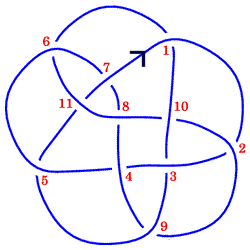
\includegraphics[width=0.6\linewidth]{../data/mixed/gauss_code.png}
        \subcaption{...dla kodu Gaußa}
    \end{minipage}
    \quad
    \begin{minipage}[b]{.45\linewidth}
        \centering
        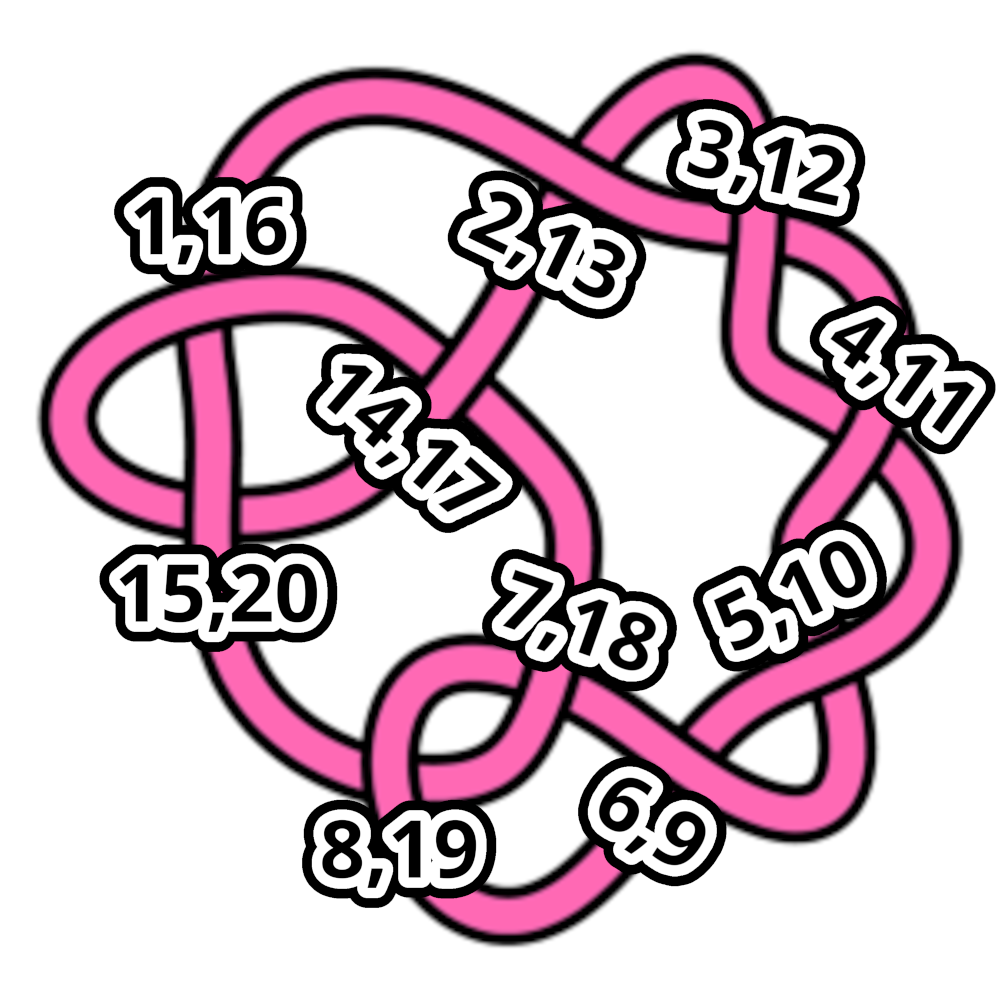
\includegraphics[width=0.6\linewidth]{../data/mixed/dowker_code.png}
        \subcaption{...dla kodu Dowkera-Thistlethwaite'a}
    \end{minipage}
    \caption[gauss-dowker-thistlethwaite]{Numeracja skrzyżowań}
    \label{gauss_dt}%
\end{figure}

% wiem o tym z "Aspects of topology, in memory of H. Dowker"
Gauß był świadomy, że szukanie koniecznych i wystarczających warunków na to, by ciąg $2n$ liczb był kodem jakiegoś węzła jest ciekawym problemem, ale chyba nie zdecydował się nim zająć.
Stosowne algorytmy podali trochę później topolodzy (Dehn \cite{dehn1936}) i dużo później teoretycy grafów (Rosenstiehl, Read \cite{rosenstiehl1978}).
Inny algorytm Dowkera, Thistlethwaite'a \cite{dowker1983} został zaimplementowany jako program komputerowy liczący około 30 linii kodu, stanowił ważny element tablicowania małych węzłów pierwszych.

\index{notacja!Gaußa|)}%

\subsubsection{Notacja Dowkera-Thistlethwaite'a}
\index{notacja!Taita}
\index{notacja!Dowkera-Thistlethwaite'a|(}
Poprawia nieopisaną tutaj notację Taita, opisana po raz pierwszy w~pracy \cite{dowker1983}.
\index[persons]{Dowker, Clifford}%
\index[persons]{Thistlethwaite, Morwen}%

Tak jak w~notacji Gaußa, przemierzamy węzeł zaczynając poza skrzyżowaniem.
Tym razem jednak stare skrzyżowania dostają drugi, nowy numer.
Jak można zauważyć, każde skrzyżowanie ma parzystą oraz nieparzystą etykietę.

\begin{definition}
    Ciąg parzystych liczb występujących na diagramie kolejno przy $1, 3, \ldots$ nazywamy kodem Dowkera-Thistlethwaite'a.
    Jeżeli nieparzysta etykieta odpowiadała podskrzyżowaniu, zapisujemy liczbę z~minusem.
\end{definition}

Opisany powyżej kod nie jest idealny, ponieważ odtworzony z niego węzeł może być lustrzanym odbiciem wyjściowego.
Ogólniej, odbicie dowolnego składnika sumy spójnej nie zmienia kodu całego węzła.
Nie stanowi to jednak dużego problemu, ponieważ notacja została stworzona na potrzeby tablicowania węzłów pierwszych, a~te są niezorientowane.

\begin{example}
    Rozpatrzmy węzeł z rysunku \ref{gauss_dt}.
    Jego kodem Dowkera-Thistlethwaite'a jest ciąg {16 12 10 18 6 4 2 20 14 8}.
\end{example}

Zaczynając od zredukowanego diagramu o $n$ skrzyżowaniach nie można doprowadzić do sytuacji, gdzie do pewnego skrzyżowania przypisane są dwie kolejne liczby całkowite.
Dzięki temu problem można przetłumaczyć na język teorii grafów.
Rozpatrzmy graf $G$, którego wierzchołkami są liczby $1, 2, \ldots, 2n$.
Połączmy niesąsiadujące modulo $2n$ wierzchołki o różnej parzystości krawędziami.
Graf ten powstaje przez usunięcie cyklu Hamiltona (łączącego kolejne liczby) z pełnego grafu dwudzielnego.
Zbiór par etykiet przy skrzyżowaniach węzła to skojarzenie doskonałe w grafie $G$.
Liczba skojarzeń prawie pokrywa się z rozwiązaniem zadania znanego w literaturze jako ,,\textsc{problème des ménages}'': na ile sposobów $n$ małżeństw można posadzić przy okrągłym stole tak, by żadne małżeństwo nie siedziało obok siebie i~każdy mężczyzna znalazł się obok dwóch kobiet?
\index{problem małżeństw przy stole}%
Ustawienia, które powstają przez cykliczne permutowanie należy uznać za tożsame.
Gilbert \cite{gilbert1956} znalazł wzór na $a_n$, liczbę różnych kodów:
\index[persons]{Gilbert, Edgar}%
\begin{align}
u(m, t) & = 2m \sum_{k=0}^m {2m-k \choose k} \cdot (m-k)! \cdot \frac{(t-1)^k}{2m - k}  \\
a(n) & = \frac{1}{n} \sum_{d\mid n} \left(\frac{n}{d}\right)^d \cdot u \left(d, 1 - \frac{d}{n}\right) \cdot \varphi \left(\frac{n}{d}\right)
\end{align}

Kilka początkowych wartości to $a_3 = 1, 2, 5, 20, 87, 616, 4843, 44128, 444621, \ldots$ (ciąg \href{https://oeis.org/A002484}{A002484} w OEIS).

\index{notacja!Dowkera-Thistlethwaite'a|)}%

\subsubsection{Notacja Alexandera-Briggsa}
\label{alexander_briggs_notation}%
\index{notacja!Alexandera-Briggsa|(}%
W~1927 roku Alexander, Briggs wprowadzili zupełnie inny sposób oznaczania węzłów -- wtedy do 9 skrzyżowań, ale przedłużony do 10 skrzyżowań przez Rolfsena i używany po dziś dzień.
Do opisu węzła używa się dwóch liczb: jego indeksu skrzyżowaniowanego z dolnym indeksem, oznaczającym miejsce w tablicy~węzłów.
I~tak węzły o~ośmiu skrzyżowaniach to $8_1, 8_2, \ldots,$ $8_{21}$.
Porządek jest umowny i jego wybór należy do osoby, która jako pierwsza znajdzie wszystkie węzły o danej liczbie skrzyżowań (ale węzeł skręcony występuje zawsze po torusowym).
% TODO: dlaczego?
\index{węzeł!skręcony}%
\index{węzeł!torusowy}%

Od jedenastu skrzyżowań pojawia się mała zmiana: węzły alternujące i niealternujące kataloguje się osobno.
I tak $11n_{185}$ to sto osiemdziesiąty piąty węzeł niealternujący o 11 skrzyżowaniach, zaś $11a_{367}$ to trzysta sześćdziesiąty siódmy alternujący.

Rolfsen w 1976 stworzył z kilkoma błędami tablicę diagramów pierwszych węzłów do 10 skrzyżowań.
\index[persons]{Rolfsen, Dale}%
\label{rolfsens_mistake}%
Para Perko $10_{161}, 10_{162}$ przedstawia ten sam węzeł, zaś górne skrzyżowanie w~$10_{144}$ powinno być zmienione.
\index{para Perko}%
Ostatnie cztery węzły dostały nowe numery, by uniknąć duplikatu.
Kolejną usterką tablicy jest to, że notacja Conwaya oraz wielomian Alexandera dla węzłów $10_{83}$ oraz $10_{86}$ są zamienione miejscami.
Tu czyha pułapka:\footnote{Wiemy o niej dzięki stronie \url{http://stoimenov.net/stoimeno/homepage/ptab/}.} Stojmenow, nowe wydanie książki Rolfsena, atlas węzłów Bar-Natana oraz tablica niezmienników węzłowych Livingstona naprawiają to przez wymianę podpisów.
Podręcznik Kawauchiego wymienia diagramy.

Ze strony internetowej Stojmenowa dowiedzieliśmy się jeszcze czegoś.
Kolejność Rolfsena dla węzłów o 10 skrzyżowaniach obala nomenklaturę Little'a niealternujących oraz nadpisuje numerowanie Taita dla alternujących węzłów.
\index[persons]{Little, Charles}%
Alexander, Briggs zrobili wcześniej to samo dla 9 lub mniej skrzyżowań.

\index{notacja!Alexandera-Briggsa|)}%

\subsubsection{Notacja Conwaya}
\index{notacja!Conwaya}%
Wprowadzona przez Conwaya w~pracy \cite{conway1970}.
Wymaga znajomości supłów, więc przedstawiamy ją po ich zdefiniowaniu, na stronie \pageref{conway_notation}.

\subsubsection{Nazwy zwyczajowe}
\label{sssec:link_names}%
Niektóre węzły i sploty, w szczególności te o niskim indeksie skrzyżowaniowym, występują tak często w teorii węzłów, że doczekały się nazw zwyczajowych.
Oto ich lista:
\begin{compactitem}
% DICTIONARY;unknot;niewęzeł;-
% TODO: nigdzie w książce nie ma definicji niesplotu?
    \item węzeł $0_1$ to niewęzeł;
\index{niewęzeł}%
% DICTIONARY;trefoil knot;trójlistnik;-
    \item węzeł $3_1$ to trójlistnik,
\index{trójlistnik}%
% DICTIONARY;figure-eight;ósemka;-
    \item węzeł $4_1$ to ósemka albo węzeł Listinga,
\index{ósemka}%
% DICTIONARY;cinquefoil knot;pięciolistnik;-
    \item węzeł $5_1$ to pięciolistnik albo węzeł Solomona (!),
\index{pięciolistnik}%
\index{węzeł Solomona}%
% DICTIONARY;stevedore knot;węzeł dokerski;-
    \item węzeł $6_1$ to węzeł dokerski/sztauerski,
\index{węzeł dokerski}%
    \item węzeł 11n34 to węzeł Conwaya,
\index{węzeł Conwaya}%
    \item węzeł 11n42 to węzeł Kinoshity-Terasakiego,
\index{węzeł Kinoshity-Terasakiego}%
    \item węzeł 12n242, czyli $(-2, 3, 7)$-precel, to z powodu pracy \cite{fintushel1980} węzeł  Fintushela-Sterna,
\index{węzeł Fintushela-Sterna}%
\index[persons]{Fintushel, Robert}%
\index[persons]{Stern, Robert}%
% DICTIONARY;granny knot;węzeł babski;-
    \item suma spójna takich samych trójlistników to węzeł babski,
\index{węzeł babski}
% DICTIONARY;square knot;węzeł prosty/płaski
    \item suma spójna lustrzanych trójlistników to, dość niefortunnie, węzeł prosty/płaski % (dość niefortunna nazwa),
% TODO: nigdzie w ksiażce nie ma definicji notacji A-B dla splotów?
    \item splot $2_1^2$ (L2a1) to splot Hopfa,
\index{splot Hopfa}%
    \item splot $4_1^2$ (L4a1) to węzeł Solomona (!),
\index{węzeł Solomona}%
    \item splot $5_1^2$ (L5a1) to splot Whiteheada,
\index{splot Whiteheada}%
    \item splot $6_2^3$ (L6a4) to pierścienie Boromeuszy.
\index{pierścienie Boromeuszy}%
\end{compactitem}



